% ---------------------------------------------------------------
% report_quantum_mpemba_ja.tex   (Japanese version)
%
% Compile with LuaLaTeX:
%     latexmk -lualatex report_quantum_mpemba_ja.tex
%
% Layout constraints imposed by the assignment:
%     A4 / one column / 11pt body / 25mm margins on all four sides
%     main text within 8 pages (figures and tables included);
%     bibliography and appendices do NOT count towards the 8 pages.
%
% Notation lives in macros.tex and is shared with the English version.
% ---------------------------------------------------------------
\documentclass[a4paper,11pt,onecolumn]{jlreq}

\usepackage[margin=25mm]{geometry}
\usepackage{amsmath,amssymb}
\usepackage{physics}
\usepackage{graphicx}
\usepackage{booktabs}
\usepackage{listings}
\usepackage[hidelinks]{hyperref}

% ---------------------------------------------------------------
% macros.tex
% Shared notation for the Japanese and English versions of the report.
% Both versions MUST \input this file so that the two documents use
% literally the same symbols.  Do not define notation anywhere else.
%
% Naming policy: avoid every control sequence already provided by the
% `physics' package (\tr, \Tr, \dd, \dv, \pdv, \qty, \abs, \norm,
% \expval, \ev, \comm, \acomm, \pb, \order, ...).
% ---------------------------------------------------------------

% --- Unified description ----------------------------------------
% The report treats a classical probability vector and a density matrix on the
% same footing; \vstate denotes either, and \gen denotes whichever generator
% acts on it.  These two symbols carry the unification of the three papers.
\newcommand{\vstate}{\varrho}           % unified state: p(t) classically, rho(t) quantum mechanically
\newcommand{\gen}{\mathcal{G}}          % unified generator: R classically, \Lop quantum mechanically
\newcommand{\ssv}{\vstate_{\mathrm{ss}}}% unified stationary state
\newcommand{\ipr}[2]{\langle #1 , #2 \rangle} % duality pairing between left and right modes

% --- Generators of the dynamics ---------------------------------
\newcommand{\Lop}{\mathcal{L}}          % Lindbladian / Liouvillian superoperator
\newcommand{\Rmat}{R}                   % classical Markov rate matrix (notation of Lu-Raz)
\newcommand{\Wmat}{\mathsf{W}}          % classical Markov rate matrix (generic)
\newcommand{\jump}{L}                   % Lindblad jump operator

% --- Stationary states ------------------------------------------
\newcommand{\pss}{\pi}                  % classical stationary distribution
\newcommand{\rss}{\rho_{\mathrm{ss}}}   % quantum steady state

% --- Spectral decomposition -------------------------------------
\newcommand{\reig}[1]{r_{#1}}           % right eigenvector (eigenmode) of the generator
\newcommand{\leig}[1]{\ell_{#1}}        % left eigenvector, dual to \reig
\newcommand{\ovl}[1]{a_{#1}}            % overlap coefficient of the initial state with mode #1
\newcommand{\gap}{\lambda_{2}}          % spectral gap: slowest decaying nonzero mode

% --- Temperatures -----------------------------------------------
\newcommand{\betaeff}{\beta_{\mathrm{eff}}}   % effective inverse temperature
\newcommand{\betabath}{\beta_{\mathrm{bath}}} % inverse temperature of the bath
\newcommand{\betainit}{\beta_{0}}             % initial inverse temperature (state preparation)

% --- Keldysh Green's functions ----------------------------------
\newcommand{\Gret}{G^{R}}               % retarded Green's function
\newcommand{\Gadv}{G^{A}}               % advanced Green's function
\newcommand{\Gkel}{G^{K}}               % Keldysh Green's function
\newcommand{\Ggtr}{G^{>}}               % greater Green's function
\newcommand{\Glss}{G^{<}}               % lesser Green's function
\newcommand{\Sret}{\Sigma^{R}}          % retarded self-energy
\newcommand{\Sgtr}{\Sigma^{>}}          % greater self-energy

% --- Model parameters -------------------------------------------
\newcommand{\Jsyk}{J}                   % SYK four-fermion coupling
\newcommand{\Vsb}{V}                    % system-bath coupling
\newcommand{\hyb}{\Gamma}               % hybridisation function of the resonant level
\newcommand{\bandw}{\Lambda}            % bath bandwidth (Lorentzian half-width)
\newcommand{\edot}{\varepsilon_{d}}     % energy of the resonant level

% --- Distance measures ------------------------------------------
\newcommand{\Dbath}{D_{\mathrm{bath}}}  % distance from the asymptotic bath distribution
\newcommand{\Deq}{D_{\mathrm{eq}}}      % distance from the equilibrium state at the same \betaeff

% --- Miscellaneous ----------------------------------------------
% House style: the differential is upright (\dd from `physics'), while the
% imaginary unit and Euler's number stay italic.  The macros below exist so
% that this convention is applied uniformly and can be changed in one place.
\newcommand{\ii}{i}                     % imaginary unit (italic, per house style)
\newcommand{\ee}{e}                     % Euler's number (italic, per house style)
\newcommand{\Feq}{f_{\mathrm{eq}}}      % Fermi-Dirac distribution
\newcommand{\Feff}{f_{\mathrm{eff}}}    % nonequilibrium (effective) distribution function


% Code listings for the appendix (Python).
\lstset{
  basicstyle=\ttfamily\footnotesize,
  keywordstyle=\bfseries,
  commentstyle=\itshape,
  frame=single,
  breaklines=true,
  showstringspaces=false,
  language=Python
}

% TODO: fill in the author name before submission.  The submitted PDF must be
% named after the author, as required by the assignment.
\title{量子ムペンバ効果の起源\\
---スペクトル機構と動的機構の統一的記述と分離---}
\author{川合玲央}
\date{\today}

\begin{document}
\maketitle

\begin{abstract}
ムペンバ効果の起源をめぐる二つの整合しない描像を，共通の記法のもとで一貫した議論として再構成する．
Lu--Raz\cite{Lu2017}による古典Markov過程の定式化とCarolloら\cite{Carollo2021}によるLindblad方程式への拡張は，緩和生成子のスペクトル分解における最緩和モードとの重なり係数$\ovl{2}$で現象を特徴づける点で同一の構造をもつ（\emph{スペクトル機構}）．
一方Wangら\cite{Wang2024}は，強結合SYK模型において温度軌跡の交差が系--浴結合$\Vsb$のみに支配され初期条件に依存しないことを示した（\emph{動的機構}）．
本レポートは，この対立が「時間局所的な生成子が存在するか否か」の一点に帰着することを示し，三状態Markov模型と共鳴準位模型により動的機構が相互作用にもカオス性にも依存しないことを検証したうえで，実効温度の定義依存性という観点から\cite{Wang2024}の限界を批判的に検討して未解決問題を提示する．
\end{abstract}

% ===============================================================
\section{Introduction}
\label{sec:intro}
% ---------------------------------------------------------------

高温の水が低温の水よりも速く凍るというムペンバ効果\cite{Mpemba1969}は，準静的熱力学では説明できない緩和現象の代表例である．
準静的な描像では冷却速度は状態量の関数であり，異なる初期温度から出発した温度軌跡が交差することは許されない．
したがって温度軌跡の交差（Mpemba crossing，以下MPC）は，緩和過程が平衡状態の系列としては記述できないことの直接的な証拠となる\cite{Lu2017}．

この現象に理論的基礎を与えたのがLu--Raz\cite{Lu2017}である．
彼らはMarkov的緩和において，確率分布を遷移速度行列の固有モードに分解したときの第二モードの係数$\ovl{2}$が緩和の遅さを支配することを見出し，ムペンバ効果の十分条件を導いた．
要点は，緩和の速さが\emph{初期状態と特定の固有モードとの幾何学的な重なり}に還元される点にある．
Carolloら\cite{Carollo2021}はこの構造がLindblad方程式にそのまま移植できることを示し，最緩和モードに直交させるユニタリ変換を緩和開始直前に施すことで緩和を指数関数的に加速できるという\emph{制御プロトコル}を提案した（可積分系での関連研究として\cite{Ares2023,Rylands2024}）．

これらはいずれもMarkov近似---浴の相関時間が零で系--浴結合が弱いこと---に立脚し，扱う模型も可積分あるいは少数自由度の系に限られるため，古典実験で本質的とされる冷却の\emph{速さ}が理論の中で役割を果たさない．
さらに深刻なのは，Hamiltonianがランダム行列として振る舞う量子カオス系では初期状態の情報が急速にスクランブルされ\cite{Maldacena2016}，微調整された初期状態の特別さが失われて$\ovl{2}$に基づく議論の前提そのものが崩れうるという点である．

Wangら\cite{Wang2024}はこの空白を埋める．
彼らはSYK模型を強結合のSYK浴に結合させた系のクエンチダイナミクスをKadanoff--Baym方程式で厳密に解き，(i)MPCが結合$\Vsb$の閾値を超えたときにのみ現れその閾値が初期条件に依存しないこと，(ii)同じ模型をLindblad方程式で記述するとMPCが消失すること，(iii)二浴の温度差はMPCをむしろ抑制すること---可積分系での既知の結果\cite{WangWang2024}と逆である---を示した．
(ii)は本レポートの議論にとって決定的である．
Lindblad記述はまさに\cite{Carollo2021}の枠組みが厳密に成立する状況であり，そこでMPCが消えるという事実は，二つの機構が同じ現象の異なる説明ではなく\emph{異なる現象}であることを意味する．
Wangらの新規性は，初期条件機構が原理的に働かない量子カオス系を舞台に選び，非平衡ダイナミクス自体が交差を生むことを示した点にある．
以下，第\ref{sec:model}--\ref{sec:results}節で三つの設定と主張を共通の記法で捉え直し（背景は付録\ref{sec:appendix_prelim}），第\ref{sec:minimal}節で最小模型による検証，第\ref{sec:discussion}節で仮定の限界の検討，第\ref{sec:open}節で未解決問題の提示を行う．

% ===============================================================
\section{Model}
\label{sec:model}
% ---------------------------------------------------------------

\subsection{統一的記述の設定}
\label{sec:model_unified}

系は時刻$t=0$に逆温度$\betainit$の平衡状態$\vstate(0)$に用意され，その後に逆温度$\betabath$の浴と接触して緩和するものとする．
状態$\vstate$は古典的には確率分布$p(t)$，量子的には密度行列$\rho(t)$を表す統一記号である．
時間発展が時間非依存の生成子$\gen$によって
\begin{equation}
  \dv{\vstate(t)}{t} = \gen\,\vstate(t)
  \label{eq:generator}
\end{equation}
と生成されるとき，$\gen$の固有値を$\lambda_1=0>\Re\lambda_2\ge\Re\lambda_3\ge\cdots$と並べ，右固有モードを$\reig{k}$，左固有モードを$\leig{k}$，双対性を$\ipr{\leig{k}}{\reig{h}}=\delta_{kh}$とする．
このとき\eqref{eq:generator}の解は
\begin{equation}
  \vstate(t) = \ssv + \sum_{k\ge2}\ovl{k}\,\ee^{\lambda_k t}\,\reig{k}\,,
  \qquad
  \ovl{k} = \ipr{\leig{k}}{\vstate(0)}
  \label{eq:spectral_unified}
\end{equation}
と分解される．
$\ssv$は$\gen\ssv=0$を満たす定常状態，$\ovl{k}$は初期状態と第$k$モードとの重なりであり，この係数$\ovl{k}$が以下の議論全体の中心となる．

古典Markov過程では$(\reig{k},\leig{k})$は遷移速度行列$\Rmat$の右・左固有ベクトルで対$\ipr{\cdot}{\cdot}$はベクトルの内積，Lindblad方程式では$\reig{k},\leig{k}$は$\Lop$と随伴$\Lop^{\dagger}$の固有行列で対はHilbert--Schmidt内積$\ipr{\leig{k}}{\rho}=\tr[\leig{k}\rho]$となり\cite{Carollo2021}，\eqref{eq:spectral_unified}はこの両方を含む．
すなわち
\begin{align}
  \text{古典：}\quad \dot{p} &= \Rmat\,p\,, &
  \text{量子：}\quad \dot{\rho} &= \Lop[\rho]
    = -\ii\comm{H}{\rho}
      + \sum_{\mu}\left(\jump_\mu \rho \jump_\mu^{\dagger}
      - \frac{1}{2}\acomm{\jump_\mu^{\dagger}\jump_\mu}{\rho}\right)
  \label{eq:two_generators}
\end{align}
であり，両者は\eqref{eq:spectral_unified}という同一の構造を共有する．

\subsection{生成子が存在しない場合：強結合SYK}
\label{sec:model_syk}

Wangら\cite{Wang2024}が扱うのは\eqref{eq:generator}の前提が成り立たない状況であり，$N$個のMajorana fermion $\chi_i$からなる系を，$N^2$個のMajorana fermion $\psi_i$からなるSYK$_4$浴（付録\ref{sec:appendix_syk}）に結合させた
\begin{equation}
  H = H_{\mathrm{SYK}}[J,\chi] + H_{\mathrm{SYK}}[\tilde{J},\psi]
    + \sum_{a i_1\cdots i_n}\frac{V_{a i_1 \cdots i_n}}{n!}\,
      \chi_a \psi_{i_1}\psi_{i_2}\cdots\psi_{i_n}
  \label{eq:H_coupled}
\end{equation}
を考える（$H_{\mathrm{SYK}}[J,\chi]$は付録\eqref{eq:H_syk_pure}と同形）．
結合定数は平均零のGauss分布に従い，分散は独立に
\begin{align}
  \overline{J_{i_1 i_2 i_3 i_4}^{\,2}} &= \frac{3!\,\Jsyk^2}{N^3}\,, &
  \overline{\tilde{J}_{i_1 i_2 i_3 i_4}^{\,2}} &= \frac{3!\,\Jsyk^2}{N^6}\,, &
  \overline{V_{a i_1 \cdots i_n}^{\,2}} &= \frac{n!\,\Vsb^2}{N^{2n}}
  \label{eq:variances}
\end{align}
で与えられる．
浴の自由度が系の$N$倍のオーダーで多いため浴は温度$\betabath^{-1}$を保つ理想的な熱浴として振る舞う．
この系のクエンチダイナミクスはKeldysh輪郭上のKadanoff--Baym方程式
\begin{equation}
  \begin{split}
    \ii\,\partial_{t_1}\Ggtr(t_1,t_2)
      &= \int \dd{t_3}\Big[\Sret(t_1,t_3)\,\Ggtr(t_3,t_2)
        + \Sgtr(t_1,t_3)\,\Gadv(t_3,t_2)\Big]\,,\\
    -\ii\,\partial_{t_2}\Ggtr(t_1,t_2)
      &= \int \dd{t_3}\Big[\Gret(t_1,t_3)\,\Sgtr(t_3,t_2)
        + \Ggtr(t_1,t_3)\,\Sigma^{A}(t_3,t_2)\Big]
  \end{split}
  \label{eq:kadanoff_baym}
\end{equation}
で記述され，自己エネルギーは$\Sigma_\chi\sim\Jsyk^2 G_\chi^3+\Vsb^2 G_\psi^n$の形をとる．
右辺には過去の全履歴にわたる時間積分，すなわち記憶項が現れる．
これが決定的な差異である．
\eqref{eq:kadanoff_baym}は\eqref{eq:generator}のような時間局所的な形に書けず，したがって\eqref{eq:spectral_unified}のスペクトル分解も重なり係数$\ovl{k}$も定義できない．
三つの設定の対応関係を表\ref{tab:unification}にまとめる．

\begin{table}[htbp]
  \centering
  \caption{三つの研究の統一的対応関係．
           上二段は\eqref{eq:spectral_unified}という同一の構造をもち，
           最下段のみ時間局所的な生成子が存在しないためスペクトル分解が定義できない．}
  \label{tab:unification}
  \small
  \begin{tabular}{@{}lllll@{}}
    \toprule
    文献 & 生成子$\gen$ & 双対対$\ipr{\cdot}{\cdot}$ & 制御変数 & 機構 \\
    \midrule
    Lu--Raz\cite{Lu2017}
      & 速度行列$\Rmat$ & ベクトル内積
      & $\ovl{2}(\betainit)$ & スペクトル \\
    Carolloら\cite{Carollo2021}
      & Lindbladian $\Lop$ & $\tr[\leig{2}\rho]$
      & $\ovl{2}=\tr[\leig{2}U\rho_0 U^{\dagger}]$ & スペクトル \\
    Wangら\cite{Wang2024}
      & 存在しない（記憶項） & ---
      & 結合強度$\Vsb/J_0$ & 動的 \\
    \bottomrule
  \end{tabular}
\end{table}

% ===============================================================
\section{Results}
\label{sec:results}
% ---------------------------------------------------------------

\subsection{スペクトル機構：古典的定式化と量子的拡張}
\label{sec:results_spectral}

Lu--Raz\cite{Lu2017}は初期分布を逆温度$\betainit$のGibbs分布に取ることで$\ovl{k}$を$\betainit$の関数とみなす．
長時間では\eqref{eq:spectral_unified}の和は最緩和モード$k=2$に支配されるから，定常状態への接近の遅さは$\abs{\ovl{2}(\betainit)}$で決まる．
高温側の初期逆温度を$\betainit^{h}$，低温側を$\betainit^{c}$（$\betainit^{h}<\betainit^{c}$）とすると，ムペンバ効果の十分条件は
\begin{equation}
  \lambda_2 > \lambda_3
  \quad\text{かつ}\quad
  \abs{\ovl{2}^{\,c}} > \abs{\ovl{2}^{\,h}}
  \label{eq:mpemba_condition}
\end{equation}
と表される．
第一条件は最緩和モードの一意性を，第二条件は高温の初期状態のほうが遅いモードとの重なりが小さいことを要求し，同じ論法を加熱に適用すると$\abs{\ovl{2}^{\,h}}>\abs{\ovl{2}^{\,c}}$のもとでの逆ムペンバ効果（低温の系がより速く加熱される）が予言される（一次元拡散過程と三状態系で例示）．

Carolloら\cite{Carollo2021}は\eqref{eq:spectral_unified}をLindblad系に適用し，形式解
$\ee^{t\Lop}[\rho_0]=\rss+\sum_{k\ge2}\ee^{t\lambda_k}\tr[\leig{k}\rho_0]\reig{k}$
を出発点として，定常状態からの隔たりをHilbert--Schmidt距離$\mathcal{E}_t(\rho,\rss)=(\tr[(\ee^{t\Lop}[\rho]-\rss)^2])^{1/2}$で測る．
その長時間漸近形は$\abs{\ovl{2}}\ee^{\Re\gap t}$に比例し，緩和時間は$\tau=1/\abs{\gap}$である．
ここで彼らはLu--Razから一歩踏み込み，初期状態を受動的に選ぶのではなく，緩和開始直前にユニタリ変換$U$を施して能動的に$\ovl{2}$を消す．
すなわち
\begin{equation}
  \tr\!\left[\leig{2}\,U\rho_0 U^{\dagger}\right] = 0
  \label{eq:optimal_unitary}
\end{equation}
を満たす$U$を構成すると，緩和は第三モードに支配され，因子$\ee^{\,t(\abs{\Re\lambda_3}-\abs{\Re\gap})}$で指数関数的に加速される．
彼らはこれをDicke模型と全対全相互作用スピン系で実証し，後者では一次転移近傍の準安定領域を回避できることを示した．
\eqref{eq:optimal_unitary}の実行には$\leig{2}$を陽に知っていることが必要であり，この要請はカオス系では原理的に満たされない．

\subsection{動的機構：強結合SYK模型}
\label{sec:results_wang}

Wangら\cite{Wang2024}は\eqref{eq:H_coupled}のクエンチダイナミクスを\eqref{eq:kadanoff_baym}で数値的に解き，ゆらぎ--応答関係に基づく実効温度$\betaeff(t)$（定義は付録\ref{sec:appendix_prelim}）を\eqref{eq:beta_eff}に従って追跡した．

弱結合では$\betaeff(t)$は
\begin{equation}
  \betaeff(t) \simeq \beta_f + \alpha\,\ee^{-\Gamma t}
  \label{eq:slow_relaxation}
\end{equation}
という単調な指数緩和を示す\cite{Eberlein2017}．
ここで$\beta_f$は終状態の逆温度，$\alpha$は初期・終状態の温度差に関係する定数，$\Gamma$は初期状態に依存しない緩和率であり，この形は準静的熱力学と整合して交差を許さない．
ところが$\Vsb$が閾値を超えると$\betaeff(t)$は定常値のまわりで振動してMPCが現れ，さらに強い結合では負の実効温度を与える領域さえ生じる．
決定的なのは，この閾値を決めるのが初期条件ではなく$\Vsb$のみだという点であり，\eqref{eq:mpemba_condition}の$\ovl{2}(\betainit)$による条件づけとは対照的である．

同じ模型をLindblad方程式で記述するとMPCは消失する．
Lindblad記述は無限温度の浴に弱く結合したSYK模型に相当するが，厳密計算ではGreen関数が無限温度でも$\Jsyk$に比例する有限の幅をもつのに対し，Lindblad近似はこれをDirac delta関数で置き換えてしまい，浴の記憶を捨てた瞬間に現象が消える．
また二浴の温度差を大きくすると閾値結合はむしろ増大し，可積分系で温度差がムペンバ効果を促進する結果\cite{WangWang2024}と逆で，機構の差異を示す独立な証拠となる．

\subsection{統一的解釈}
\label{sec:results_synthesis}

スペクトル機構が意味をもつのは$\gen$が存在し$\ovl{2}$が定義できる場合，すなわちMarkov極限に限られる．
この極限では異常緩和は初期状態と特定モードの幾何学的関係に還元され，冷却の速さ自体は本質的な役割を果たさない．
動的機構が現れるのはこの極限が破れる強結合領域であり，記憶項が無視できなくなると$\ovl{2}$は定義を失って，代わりに$\Vsb$が制御する緩和の速さが現象を支配する．
したがって二つの機構は矛盾するのではなく\emph{排他的}であり，\cite{Wang2024}がLindblad SYKでMPCを見出せなかったのはその直接的な帰結である．
逆に\cite{Carollo2021}の制御プロトコル\eqref{eq:optimal_unitary}はSYK模型では二重の意味で実行不能である．
$\leig{2}$がそもそも定義されず，仮に定義されたとしても無秩序平均されたアンサンブル理論において特定の$\leig{2}$を狙うことはできない．

% ===============================================================
\section{Minimal Model and Test}
\label{sec:minimal}
% ---------------------------------------------------------------

前節の解釈を検証するため二つの最小模型を設定する．
第\ref{sec:minimal_markov}節ではスペクトル機構を，第\ref{sec:minimal_rlm}節では動的機構を，それぞれ厳密に扱える最小の設定で再現する．
特に後者では，動的機構が\emph{相互作用にもカオス性にも依存しない}ことを示す．

\subsection{三状態Markov模型}
\label{sec:minimal_markov}

エネルギー$E_1<E_2<E_3$をもつ三準位系が逆温度$\betabath$の浴と接触する状況を考える．
遷移速度行列$\Rmat$は詳細釣り合い$\Rmat_{ij}\ee^{-\betabath E_j}=\Rmat_{ji}\ee^{-\betabath E_i}$（$i\neq j$）と確率保存$\sum_i\Rmat_{ij}=0$を満たすものとする．
三準位は\cite{Lu2017}が例示に用いた最小の離散系であり，$\Rmat$が$3\times3$であるため固有値と左右固有ベクトルを容易に求められる．

$\Rmat$を対角化して$\lambda_2,\lambda_3$と$\leig{2}$を求め，初期分布を逆温度$\betainit$のGibbs分布に取って$\ovl{2}(\betainit)=\ipr{\leig{2}}{\vstate(0)}$を計算し，その符号反転をまたぐ二つの初期温度から緩和させる．
パラメータ$E=(0,1,5)$，$\Gamma=(0.3,2.0,0.001)$，$\betabath=0.5$は，$\lambda_2>\lambda_3$と$\ovl{2}$の第二の零点の存在を条件に走査して選んだ．

結果を図\ref{fig:markov_a2}に示す．
固有値は$\lambda_2=-0.600$，$\lambda_3=-7.575$（ギャップ比$12.6$）で，$\ovl{2}$は$\betabath$のほかに$\betainit^{*}=0.125$でも零となる．
$\betainit^{h}=0.100$と$\betainit^{c}=0.294$から出発させると$\abs{\ovl{2}}$はそれぞれ$0.0110$と$0.0330$であり，高温側は初期時刻で定常状態から\emph{より遠い}にもかかわらず（$L^1$距離で$0.388$対$0.172$），$t=0.31$で低温側を追い越して$\norm{\vstate(t)-\ssv}_1<10^{-3}$に$t=3.93$対$t=5.76$で到達する．
これは\eqref{eq:mpemba_condition}の予言そのものである．
さらに$\betainit=\betainit^{*}$では$\ovl{2}=0$のため緩和が$\lambda_3$に支配され，同じ閾値に$t=0.78$で到達する．
これが強ムペンバ効果である．

\begin{figure}[htbp]
  \centering
  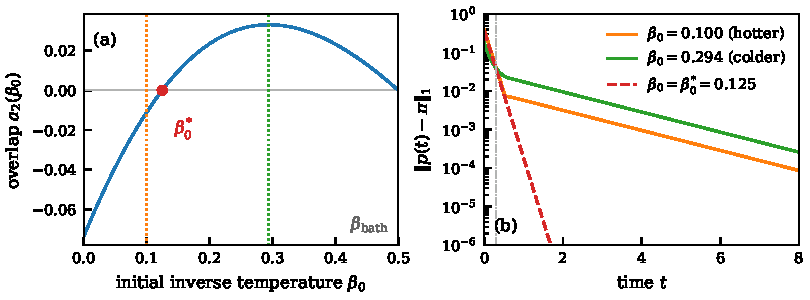
\includegraphics[width=0.85\linewidth]{figs/markov_a2.pdf}
  \caption{三状態Markov模型による検証（$E=(0,1,5)$，$\Gamma=(0.3,2.0,0.001)$，$\betabath=0.5$）．
           （a）$\ovl{2}$の初期逆温度依存性．$\betabath$のほかに$\betainit^{*}=0.125$（赤点）でも零となる．点線は（b）の初期温度．
           （b）定常状態への$L^1$距離．高温側（橙）は初期に低温側（緑）より遠いが$t=0.31$（灰破線）で追い越す．赤破線は$\betainit=\betainit^{*}$の強ムペンバ効果．}
  \label{fig:markov_a2}
\end{figure}

\subsection{共鳴準位模型}
\label{sec:minimal_rlm}

\cite{Wang2024}の主張の本質が相互作用やカオス性ではなく\emph{強結合と浴の有限相関時間}にあるならば，相互作用を完全に落とした自由フェルミオン系でも同じ現象が再現されるはずである．
これを確かめるため，単一の共鳴準位が連続的なフェルミオン浴に結合した模型
\begin{equation}
  H = \edot\, d^{\dagger} d
    + \sum_k \epsilon_k\, c_k^{\dagger} c_k
    + \sum_k \left(V_k\, d^{\dagger} c_k + \mathrm{h.c.}\right)
  \label{eq:H_rlm}
\end{equation}
を設定する．
$d$は系の準位の消滅演算子，$\edot$はその準位エネルギー，$c_k$は浴のモード$k$の消滅演算子，$V_k$は両者の混成振幅である．
この模型は二次形式であるためKeldysh Green関数が厳密に求まり，\eqref{eq:beta_eff}と\emph{同一の定義}で$\betaeff(t)$を計算できる．
すなわち\cite{Wang2024}と観測量を揃えたまま相互作用だけを取り除いた対照実験になっている．

浴の性質は混成関数
\begin{equation}
  \hyb(\omega) = \pi\sum_k \abs{V_k}^2\,\delta(\omega-\epsilon_k)
  = \frac{\hyb_0\,\bandw^2}{\omega^2+\bandw^2}
  \label{eq:hybridization}
\end{equation}
に集約される．
$\hyb_0$は結合強度，$\bandw$はLorentz型バンドの半値幅であり，浴の相関時間$\tau_{\mathrm{b}}\sim1/\bandw$を制御する唯一のパラメータである．
$\bandw\to\infty$の広帯域極限では$\tau_{\mathrm{b}}\to0$となり運動方程式は時間局所的なLindblad形式に厳密に帰着する．すなわち第\ref{sec:results_spectral}節の枠組みが成立する状況にほかならない．
逆に$\bandw$が有限であれば\eqref{eq:kadanoff_baym}と同様の記憶項が現れる．
したがって$(\hyb_0,\bandw)$平面を走査すれば，Markov極限から強結合非Markov領域までを単一の模型内で連続的に補間できる．

検証すべき予言は三点である．
(i)$\bandw$が大きい極限では$\betaeff(t)$は\eqref{eq:slow_relaxation}型の単調緩和を示し軌跡は交差しない．
(ii)$\bandw$が有限かつ$\hyb_0$が閾値を超えると$\betaeff(t)$は振動しMPCが生じる．
(iii)その閾値は初期温度$\betainit$に依存しない．

$\edot=1$，$\hyb_0=1$，$\betabath=0.25$とし，$\betainit\in\{0.02,\,0.20\}$（いずれも浴より高温）から出発させた結果を図\ref{fig:rlm_beta_eff}に示す．
$\betaeff$は\eqref{eq:beta_eff}のFDT形$\tanh(\beta\omega/2)$への最良フィットとして定め，弱結合で$\betaeff(t\to\infty)$が$\betabath$に相対誤差$5\times10^{-5}$で一致することを確認した上で用いた．

予言(i)と(ii)は確認された．
$\bandw=20$では$\betaeff(t)$は単調に$0.24997$へ収束して$\betabath$と4桁一致し，交差は生じない．
$\bandw=1$では$\betaeff(t)$は定常値のまわりで大きく振動し，負の値をとる領域さえ現れる．
この模型は二次形式であり相互作用も無秩序もスクランブルもないから，\cite{Wang2024}が報告した現象論の発現に量子カオス性は\emph{必要でない}．

しかし予言(iii)は支持されなかった．
$\betaeff$はFDTフィットに用いる周波数窓に強く依存し，$\bandw=1$の過渡領域ではその系統的な幅が最大$1.32$に達する（図\ref{fig:rlm_beta_eff}(b)の帯）．
一方，異なる$\betainit$から出発した二つの軌跡の隔たりは最大でも$0.16$である．
すなわち\emph{軌跡の隔たりは温度計自身の不定性より一桁小さく}，交差を分解できない．
閾値$\hyb_0^{\mathrm{th}}$を定義することも，その$\betainit$依存性を論じることもできない．
対照的に，状態量である$\Dbath(t)$は両方の帯域幅で\emph{単調に減少する}．

\begin{figure}[htbp]
  \centering
  
\includegraphics[width=\linewidth]{figs/rlm_beta_eff.pdf}
  \caption{共鳴準位模型による検証（$\edot=1$，$\hyb_0=1$，$\betabath=0.25$）．
           （a）$\bandw=20$（Markov的）．$\betaeff$は$\betabath$に収束し構造をもたない．
           （b）$\bandw=1$．$\betaeff$は振動し負値もとる．帯はFDTフィット窓を$2.0$--$4.0$で変えたときの広がりで，二つの初期温度の軌跡の差より一桁大きい．
           （c）状態量である$\Dbath(t)$は両方の場合に単調減少する．}
  \label{fig:rlm_beta_eff}
\end{figure}

% ===============================================================
\section{Discussion}
\label{sec:discussion}
% ---------------------------------------------------------------

\subsection{スペクトル機構が要求する仮定}
\label{sec:discussion_spectral}

第\ref{sec:results_spectral}節の議論は，(i)生成子$\gen$が時間非依存であること，(ii)$\gen$が対角化可能であること，(iii)最緩和モードが一意であること，に依拠する．
(i)はMarkov近似そのものであり破れれば\eqref{eq:spectral_unified}が書けず，(ii)が破れてJordanブロックが生じると緩和は$t^m\ee^{\lambda t}$の形をとって$\ovl{2}$による特徴づけは修正を要する．
(iii)は\eqref{eq:mpemba_condition}の第一条件として明示されており，$\Re\lambda_2=\Re\lambda_3$では加速率が零となり制御プロトコルは意味を失う．

より本質的な限界は，Hilbert--Schmidt距離の漸近形が\emph{長時間}の性質にすぎない点にある．
$\ovl{2}=0$としても短時間領域では高次モードが寄与するため緩和が実際に速いかどうかは自明でなく，\cite{Carollo2021}の主張が意味をもつのは観測時間が$1/\abs{\Re\lambda_3}$より十分長い場合に限られ，本質的に短時間の現象である古典ムペンバ実験とは噛み合わない．

\subsection{実効温度の定義依存性}
\label{sec:discussion_temperature}

\cite{Wang2024}への最も重い批判は，MPCが\emph{観測量の定義に依存する見かけの現象}である可能性を排除できていない点にある．
\eqref{eq:beta_eff}の$\betaeff(t)$は平衡FDTを非平衡に外挿した量であり，実際\cite{Wang2024}自身が，系の分布関数$\Feff(\omega,t)$と浴のFermi--Dirac分布$f_{\mathrm{bath}}(\omega)$との距離
\begin{equation}
  \Dbath(t) = \int \dd{\omega}\,
  \abs{\Feff(\omega,t) - f_{\mathrm{bath}}(\omega)}
  \label{eq:distance_bath}
\end{equation}
が時間に対して\emph{単調に減少する}ことを報告している．
つまり状態そのものは単調に定常状態へ近づいているにもかかわらず$\betaeff(t)$だけが振動しており，交差が系の状態の非単調性ではなく温度計の非線形な応答に由来する可能性を強く示唆する．

\cite{Wang2024}は別の実効温度の定義でも結論が変わらないことを補足資料で示しているが，低周波数のGreen関数に依拠する定義はいずれも同種の量であり独立な検証にはなっていない．
同じ温度を示す状態でも内部状態が異なりうるという指摘も，「実効温度が状態を完全には特徴づけない」という主張であって「交差が物理的実体をもつ」ことの論証ではない．

第\ref{sec:minimal_rlm}節の結果はこの批判を定量的にする．
共鳴準位模型では$\Dbath(t)$が単調減少する一方で$\betaeff(t)$は振動し，軌跡の隔たりはフィット窓による系統的不定性より一桁小さかった．
少なくともこの模型では交差は状態ではなく温度計の性質であり，系統誤差の評価と軌跡の隔たりとの比較がMPCの実在性を主張する最小限の手続きであろう（元来のムペンバ効果も温度計の読みで定義される）．
スペクトル機構がこれを免れているのは$\ovl{2}$が状態に対して定義されているからである．

\subsection{普遍性主張の検証状況}
\label{sec:discussion_universality}

\cite{Wang2024}は結論部で，MPCの機構をスクランブル時間$\tau_S$とエネルギー緩和時間$\tau_E$の分離$\tau_S\ll\tau_E$に帰すが，OTOCもLyapunov指数$\lambda_L$も計算されておらず定量的証拠はない．
$\Vsb$を増やせば$\lambda_L$は減少するから，MPCが現れる強結合領域はむしろカオス束縛から遠ざかる可能性さえある．

第\ref{sec:minimal_rlm}節の結果はこの主張に否定的である．
共鳴準位模型は二次形式でありスクランブルもLyapunov指数も存在しないが，$\betaeff(t)$の振動と負値は\cite{Wang2024}と同様に現れ，$\tau_S\ll\tau_E$は現象の\emph{必要条件ではない}．
普遍性の根拠として提示された機構は成立せず，残るのは記憶効果と結合強度というより単純な条件である．

% ===============================================================
\section{Open Question}
\label{sec:open}
% ---------------------------------------------------------------

第\ref{sec:discussion_temperature}節から次の未解決問題を提示する．

\begin{quote}
\textbf{問題．}
強結合非Markov開放量子系において，実効温度の定義に依存しない形でMPCを特徴づける状態量は存在するか．
存在するならば，それはMarkov極限においてスペクトル機構の$\ovl{2}$にどのように帰着するか．
\end{quote}

この問題が切実であるのは，第\ref{sec:minimal_rlm}節で$\Dbath(t)$が単調減少する一方で$\betaeff(t)$が振動し，軌跡の隔たりが温度計の不定性に埋もれることを確かめたからである．
定義非依存な特徴づけが存在しなければMPCは温度計の性質にすぎず動的機構という主張は意味を失うが，存在すればMarkov極限で$\ovl{2}$に帰着し二つの機構を真に統一する量となる．
候補として記憶核の汎関数や$\Feff(\omega,t)$の高次モーメントが考えられるが，$\ovl{2}$との接続は明らかでない．

\paragraph{まとめ．}
量子ムペンバ効果をめぐる二つの対立する描像を生成子のスペクトル分解という共通言語のもとで再構成し，両者が$\gen$の存否によって排他的に棲み分けることを示した．
最小模型による検証は，スペクトル機構が$\ovl{2}$の符号反転として確認できる一方，動的機構についてはカオス性が不要であることと交差が実効温度の定義の不定性に埋もれることを明らかにし，この不定性の評価が今後の課題として残された．

% ===============================================================
\section*{Acknowledgements}
\label{sec:ack}
% ---------------------------------------------------------------

% TODO: 謝辞本文（3行程度）をここに記入する．
\vspace{3\baselineskip}

\paragraph{生成AIの利用について．}
本レポートの作成にあたり生成AI（Claude）を，文献の探索，構成案の作成と日本語表現の校正，第\ref{sec:minimal}節の数値計算コードの下書き，式変形と書誌情報の照合に利用した．
全文献の書誌情報は原論文，arXivまたはCrossrefに当たって確認した．
記述および数式の正しさに関する責任はすべて筆者が負う．

% ===============================================================
\bibliographystyle{unsrt}
\bibliography{refs}

% ===============================================================
\appendix
\section{予備知識}
\label{sec:appendix_prelim}
% ---------------------------------------------------------------

本文で前提とするSYK模型の定義と，非平衡実効温度の定義に必要なKeldysh形式の背景をまとめる．

\subsection{SYK模型}
\label{sec:appendix_syk}

SYK模型は$N$個のMajorana fermion $\chi_i$（$\{\chi_i,\chi_j\}=\delta_{ij}$）が全対全のランダム相互作用をする$(0+1)$次元の模型であり，$q=4$では
\begin{equation}
  H_{\mathrm{SYK}}[J,\chi]
  = \sum_{i_1 i_2 i_3 i_4}
    \frac{J_{i_1 i_2 i_3 i_4}}{4!}\,
    \chi_{i_1}\chi_{i_2}\chi_{i_3}\chi_{i_4}
  \label{eq:H_syk_pure}
\end{equation}
で与えられる．
結合定数$J_{i_1i_2i_3i_4}$は平均零，分散$\overline{J^2}=3!\,\Jsyk^2/N^3$のGauss分布に従うランダム変数であり，$\Jsyk$は唯一のエネルギースケールである．
この模型が有用なのは，大$N$極限で厳密に解けながら最大限にカオス的だからである．
無秩序平均は$G$--$\Sigma$作用によるレプリカ対角化を通じて実行され，大$N$極限で単一の有効作用に帰着する点が本模型の可解性の源泉である．
これにより自己エネルギーがGreen関数で閉じ，Schwinger--Dyson方程式
$G^{-1}(\ii\omega_n)=-\ii\omega_n-\Sigma(\ii\omega_n)$，$\Sigma(\tau)=\Jsyk^2 G(\tau)^3$
が得られる一方，Lyapunov指数はカオス束縛$\lambda_L\le 2\pi k_B T/\hbar$を飽和する\cite{Maldacena2016}．

本文\S\ref{sec:model_syk}で扱う系--浴結合模型では，系と浴がともにSYK$_4$型であり，同じ形のSchwinger--Dyson方程式が結合定数$\Jsyk,\tilde{\Jsyk},\Vsb$を通じて連立する．
低エネルギー極限ではSchwarzian作用に支配され，これはJT重力の境界における揺らぎと同じ形をもつ．
この対応が，SYK模型を強結合の量子カオス系であると同時にブラックホールの熱力学を調べる玩具模型たらしめている．

本レポートにとって重要なのは，このランダム性とカオス性が\emph{初期状態の特別さを消し去る}点である．
Hamiltonianがアンサンブルとして与えられる以上，特定の固有モードを狙って初期状態を用意することはできない．
これが第\ref{sec:model_syk}節で$\gen$のスペクトル分解が定義できないと論じる際の，物理的な出発点である．

\subsection{Keldysh形式と非平衡実効温度}
\label{sec:appendix_keldysh}

温度が時間に依存する非平衡状態を扱うため，実時間Keldysh形式を導入する．
時間発展はKeldysh輪郭上で定義され，未来へ向かう分枝$\mathcal{C}_+$と過去へ戻る分枝$\mathcal{C}_-$からなる．
輪郭上の演算子$\chi_\alpha(t)$（$\alpha=\pm$）に対し，輪郭順序づけられた相関関数は
\begin{equation}
  \hat{G}_{\chi,\alpha\beta}(t,t')
  = -\ii\left\langle \mathbf{T}_c\,\chi_\alpha(t)\chi_\beta(t')\right\rangle
  = \begin{pmatrix}
      G_\chi^{T}(t,t') & \Glss_\chi(t,t') \\
      \Ggtr_\chi(t,t') & G_\chi^{\tilde{T}}(t,t')
    \end{pmatrix}
  \label{eq:contour_matrix}
\end{equation}
という行列にまとめられる\cite{Wang2024}．
ここで$\mathbf{T}_c$は輪郭に沿った順序づけを表し，時間順序付き成分と反時間順序付き成分は大小Green関数によって
\begin{align}
  G_\chi^{T}(t,t') &= \theta(t-t')\,\Ggtr_\chi(t,t') + \theta(t'-t)\,\Glss_\chi(t,t')\,, \\
  G_\chi^{\tilde{T}}(t,t') &= \theta(t'-t)\,\Ggtr_\chi(t,t') + \theta(t-t')\,\Glss_\chi(t,t')
  \label{eq:T_tildeT}
\end{align}
と表される．
遅延・進延Green関数はこれらの差から
\begin{align}
  \Gret_\chi(t,t') &= \theta(t-t')\big[\Ggtr_\chi(t,t')-\Glss_\chi(t,t')\big]\,, \\
  G_\chi^{A}(t,t') &= \theta(t'-t)\big[\Glss_\chi(t,t')-\Ggtr_\chi(t,t')\big]
  \label{eq:retarded_advanced}
\end{align}
と定義される．
自己エネルギーについても同形の関係$\Sret(t,t')=\theta(t-t')[\Sgtr(t,t')-\Sigma^{<}(t,t')]$が成り立ち\cite{Wang2024}，これらが本文\eqref{eq:kadanoff_baym}のKadanoff--Baym方程式に現れる量である．

温度が時刻$t$とともに変化する場合，二時間相関関数を中心時刻$t=(t_1+t_2)/2$と相対時刻$t'=t_1-t_2$の組に取り直し，相対時刻についてのみ半区間Fourier変換
\begin{equation}
  G(\omega,t) = \int_0^{\infty}\dd{t'}\,\ee^{\ii\omega t'}\,
  G\!\left(t+\frac{t'}{2},\,t-\frac{t'}{2}\right)
  \label{eq:wigner}
\end{equation}
を行う（Wigner変換）\cite{Wang2024}．
平衡状態では，ゆらぎ--応答関係（FDT）より
\begin{equation}
  \frac{\Im\big[\Ggtr(\omega,t)+\Glss(\omega,t)\big]}{\Im\big[\Gret(\omega,t)\big]}
  = -\tanh\!\left(\frac{\beta(t)\,\omega}{2}\right)
  \label{eq:fdt_general}
\end{equation}
が成り立つ\cite{Wang2024}．
これを$\omega\to0$で展開すると，右辺は$-\beta(t)\omega/2$に近づく．
そこでWangら\cite{Wang2024}は，非平衡状態においても同じ極限操作
\begin{equation}
  \betaeff(t) = \left.
  \frac{2\,\Im\big[\Ggtr(\omega,t)+\Glss(\omega,t)\big]}
       {\omega\,\Im\big[\Gret(\omega,t)\big]}
  \right|_{\omega\to0}
  \label{eq:beta_eff}
\end{equation}
によって実効逆温度を定義する．
平衡状態では真の逆温度に一致するが，非平衡状態でこの量が系の何を反映しているかは自明でなく，本文第\ref{sec:discussion_temperature}節で批判的に検討する．

実効温度の非平衡性を特徴づけるため，本文\eqref{eq:distance_bath}の$\Dbath(t)$のほかに，同一の実効温度における平衡分布との距離
\begin{equation}
  \Deq(t) = \int \dd{\omega}\,
  \abs{\Feff(\omega,\betaeff(t)) - \Feq(\omega,\betaeff(t))}
  \label{eq:distance_eq}
\end{equation}
も定義できる\cite{Wang2024}．
ここで$\Feq(\omega,\beta)=1/(1+\ee^{\beta\omega})$は逆温度$\beta$のFermi--Dirac分布である．
\cite{Wang2024}は，$\Dbath(t)$が単調に減少する一方で$\Deq(t)$は時間に対して非単調であると報告しており，系の統計が瞬間瞬間の実効温度における平衡分布からも系統的にずれ続けることを示している．
第\ref{sec:discussion_temperature}節の批判は主に$\Dbath(t)$の単調性に基づくが，$\Deq(t)$の非単調性もまた，実効温度という一変数だけでは非平衡状態を特徴づけられないことを示す独立な傍証である．

% ===============================================================
\section{数値計算コード}
\label{sec:appendix_code}
% ---------------------------------------------------------------

第\ref{sec:minimal}節の数値計算に用いたPythonコードは，以下の公開リポジトリの\texttt{code/}以下で公開・共有可能である．

\begin{center}
  \url{https://github.com/reo-kawai/SYK_Thermodynamics}
\end{center}

\begin{itemize}
  \item \texttt{code/mpemba\_three\_state.py}, \texttt{code/run\_three\_state\_markov.py}
        --- 三状態Markov模型（第\ref{sec:minimal_markov}節，図\ref{fig:markov_a2}）．
  \item \texttt{code/resonant\_level.py}, \texttt{code/run\_resonant\_level.py}
        --- 共鳴準位模型（第\ref{sec:minimal_rlm}節，図\ref{fig:rlm_beta_eff}）．
\end{itemize}

各計算の出力（メタデータおよび生データ）は\texttt{code/out/}以下に保存されている．

\end{document}
